\documentclass[a4paper,11pt]{report}
\usepackage[utf8]{inputenc}
\usepackage[T1]{fontenc}
\usepackage{boldline,multirow,tabularx,colortbl,diagbox,makecell,fancybox}
\usepackage{amsfonts,amssymb,amsmath,mathrsfs,array,stmaryrd}
\usepackage{pgf,tikz,xcolor}
\usetikzlibrary{calc,positioning,shapes.geometric,shapes.symbols,shapes.misc, fit, calc, shapes, arrows, arrows.meta,fadings,through}
\usepackage[top=3cm, bottom=3cm, left=3cm, right=3cm]{geometry}
\usepackage{fancyhdr}
\usepackage{hyperref}

\usepackage[french]{babel}
\usepackage{appendix,listings,enumerate}
\usepackage{ifluatex}
\usepackage[backend=biber, sorting=none, style=alphabetic]{biblatex}
\usepackage{csquotes}
\usepackage[printonlyused]{acronym}
\addbibresource{refs/bibliography.bib}

\usepackage{enumitem}
\usepackage{indentfirst}
\usepackage{notoccite}

\usepackage[nodayofweek,level]{datetime}

\usepackage{dirtree}
\usepackage{forest}
\usepackage{pdfpages}

\usepackage{booktabs}
\usepackage{caption}

\usepackage{float}
\usepackage{algorithm}
\usepackage{algpseudocode}
\newtheorem{definition}{Definition}

\newcommand{\addstudent}[4]{\textbf{#1} \\ #2 \\ #3 \\ \href{mailto:#3?subject=Regarding\projecttitle}{#4}\\}
\newcommand{\addtutor}[2]{#1 \\ #2\\}
\newcommand{\addentity}[2]{\textbf{#1} & #2\\}
\newcommand{\supervisor}{René Mandiau - HDR}
\newcommand\blankpage{%
    \null
    \thispagestyle{empty}%
    \addtocounter{page}{-1}%
    \newpage}


%=========================================================================

% Complétez ici le titre de votre projet :
\def\projecttitle{
Intelligence Artificielle Appliquée au Jeu d'Othello
}
% Complétez ici le titre de votre prénom et votre nom :
\def\students{
    \addstudent{Elias BOULANGER}{INSA Hauts-de-France - ICY}{Université Polytechnique Hauts-de-France}{elias.boulanger@uphf.fr}
}

% Complétez ici votre département (décommentez la ligne correspondante) :
\def\departement{
    Département d'Informatique et de Cybersécurité
}
\newcommand\tab[1][0.6cm]{\hspace*{#1}} %Create and define tab

\definecolor{lightgray}{gray}{0.85}
\definecolor{verylightgray}{gray}{0.85}

\newcolumntype{L}[1]{>{\raggedright\arraybackslash\hspace{0pt}}p{#1}}
\newcolumntype{R}[1]{>{\raggedleft\arraybackslash\hspace{0pt}}p{#1}}
\newcolumntype{C}[1]{>{\centering\arraybackslash\hspace{0pt}}p{#1}}

\renewcommand\thesection{\arabic{section}}
\renewcommand\thesubsection{\thesection.\arabic{subsection}}

% Redefine plain style, which is used for titlepage and chapter beginnings
% From https://tex.stackexchange.com/a/30230/828
\fancypagestyle{plain}{%
    \renewcommand{\headrulewidth}{0pt}%
    \fancyhf{}%
    \fancyfoot[R]{\thepage}%
}



%------- Do not append new commands after :

\hypersetup{	
    colorlinks=false, % colorise les liens
    linkbordercolor={1 1 1},
    breaklinks=true, % permet le retour à la ligne dans les liens trop longs
    urlcolor=blue, % couleur des hyperliens 
    linkcolor=black,	% couleur des liens internes 
    citecolor=black,	% couleur des références 
    pdftitle={Intelligence Artificielle Appliquée au
    Jeu d'Othello - Rapport des Travaux Pratiques}, % informations apparaissant dans 
    pdfauthor={Elias Boulanger}, % les informations du document 
    pdfsubject={}	% sous Acrobat. 
}
\title{Urban Traffic Noise Event Detection and Classification - 7th Semester Internship Report\\ \vspace{0.5cm} \LARGE{\textbf{\projecttitle}} \vspace{0.75cm}}
\author{\students \\ \vspace{1cm} \\ Tuteur : \tutor}
\date{\today}
\RequirePackage{fancyhdr}
\pagestyle{fancy}
\renewcommand{\headrule}{}
\lhead{}
\chead{}
\rhead{}
\lfoot{}
\cfoot{}
\rfoot{\thepage}

% Set the font size for the cover page to 12pt
\fontsize{12pt}{14pt}\selectfont

\AtBeginDocument{\pagenumbering{gobble}
%\makeatletter
\noindent\begin{tikzpicture}[remember picture, overlay, shift={(current page.south west)}]
    %Images
    \node[anchor=north west] at (1.35,23.7) {
\includegraphics[height=1.6cm, keepaspectratio]{cover/meta/insa-logo.png}};
    \node[anchor=north east] at (19.65,23.8) {
\includegraphics[height=1.8cm, keepaspectratio]{cover/meta/uphf-logo.png}};
    
    \node[above = 340pt of current page.center] (rapport) {\LARGE{\textsc{Ministère de l'enseignement supérieur et de la recherche}}};
    \node[above = 280pt of current page.center] (rapport) {
        \begin{tabular}{c}
            \huge{\textsc{\textbf{I}nstitut \textbf{N}ational des \textbf{S}ciences \textbf{A}ppliquées}} \\ \huge{\textsc{des \textbf{H}auts-de-\textbf{F}rance}}
        \end{tabular}
    };
        
    % Textes
    \node[below = 10pt of current page.center] (ptitle) {\parbox{\textwidth}{\centering\huge{\textsc{\projecttitle}}}};
    \node[above = 12.5pt of ptitle.north] {\rule{15cm}{0.25mm}};
    \node[below = 12.5pt of ptitle.south] {\rule{15cm}{0.25mm}};
    
    \node[above = 90pt of ptitle] {\LARGE{\textbf{\departement}}};
    
    \node[above = 40pt of ptitle] {\huge{\textsc{\textbf{Rapport des Travaux Pratiques}}}};

    % Adding the Supervisor Title and Name just below the Date of defence
    \node[below = 5pt of ptitle, xshift = 1.3cm] at (14.7, 10) (pdate){\large{\textbf{Date:} 15 Avril 2024}};
    \node[below = 5pt of pdate, xshift = -1.3cm] (supervisorstitle) {\large{\textbf{Professeur:} \supervisor}};
    
    \node[anchor = south west, xshift = 0.65cm] at (2,2) (pstudents) {\large{\centering\begin{tabular}{lllll}\students\end{tabular}}};

\end{tikzpicture}

\newpage
\blankpage}

\AtEndDocument{\input{cover/cover_out.tex}}

% Reset the font size to 11pt
\fontsize{11pt}{13pt}\selectfont

\begin{document}

\newpage
\thispagestyle{empty}
\tableofcontents

\newpage
\chapter*{Liste des Acronymes}
\label{chap:acronymes}

\begin{acronym}
    % \acro{<acronyme>}{<signification>}
    \acro{IA}{Intelligence Artificielle}
    \acro{LSB}{Bit de Poids Faible}
    \acro{MSB}{Bit de Poids Fort}
    \acro{PdV}{Point de Vue}
    \acro{TP}{Travail Pratique}
\end{acronym}

\newpage
\thispagestyle{empty}
\listoffigures
\listoftables

\newpage
\pagenumbering{arabic}

\chapter{Introduction}
\label{chap:introduction}

Dans ce projet de \ac{TP}, nous nous sommes attachés à développer et à évaluer des algorithmes d'\ac{IA} pour le jeu d'Othello, un jeu de plateau impliquant une stratégie complexe malgré des règles apparemment simples. Othello se joue sur un damier de 64 cases avec des pions bicolores, où l'objectif est de capturer le plus grand nombre de pions adverses. Cette simplicité apparente masque une profondeur stratégique et une explosion combinatoire qui représentent un défi de taille pour la conception d'algorithmes efficaces.

Ce rapport détaille le processus de conception, d'implémentation et d'évaluation de notre système d'\ac{IA}. Nous avons adopté une approche méthodique pour modéliser le jeu, en utilisant des structures de données adaptées pour représenter efficacement le plateau et les pions. L'accent a été mis sur l'élaboration et l'amélioration de l'algorithme Minimax, ainsi que sur ses variantes, notamment les algorithmes Alpha-Beta, qui réduisent le nombre de nœuds explorés et optimisent les performances de calcul.

Nous avons également développé une fonction d'évaluation pour mesurer la qualité des positions sur le damier, intégrant diverses heuristiques comme la position des pions, la mobilité et le contrôle du plateau. Ces heuristiques ont été testées dans différentes configurations, permettant une comparaison directe de leur efficacité à travers des matchs simulés entre notre \ac{IA} et des joueurs humains (surtout quelques amis et moi), ainsi que contre d'autres configurations d'\ac{IA}. En outre, ce travail inclus la conception d'un classifieur pour évaluer la qualité des positions. 

Ce rapport présente donc non seulement les aspects techniques de notre approche, mais aussi une discussion sur les résultats obtenus, les défis rencontrés et les potentielles améliorations.

Nous conclurons sur ce que nous avons appris de ce projet, sur les perspectives et les leçons tirées de cette expérience, avec finalement un point plus personnel.
\newpage

\chapter{Analyse}
\label{chap:anal}
Notre implémentation comprend notamment une représentation binaire, aussi appelé Bitboard, les algorithmes de recherches Minimax et Alpha-Beta, et un classifieur pour prédire le résultat d'une partie en cours. Nous détaillons également les structures de données utilisées, et les algorithmes de décalage pour les coups valides. Nous avons réalisé ce projet en Python, pour des raisons de simplicité et de rapidité de développement, notamment à propos de la visualisation, et du développement du modèle de deep learning via PyTorch\footnote{PyTorch est une bibliothèque de tenseurs optimisée pour l'apprentissage profond. Voir \href{https://pytorch.org/docs/stable/index.html}{Documentation PyTorch}.}.

% Dans la littérature, un `coup` est souvent défini comme l'action des deux joueurs pendant un tour, et un `demi-coup` comme l'action d'un seul joueur. Cependant, dans le cadre de ce rapport, nous utiliserons plutôt le terme `coup` pour désigner le fait de poser un pion.


\section{Modélisation et structures de données}
\label{sec:mod}

\subsection{Structure du projet}
\label{subsec:struct}
\dirtree{%
.1 \textbf{Othello-Reversi/}.
.2 config.yaml : fichier de configuration des paramètres globaux du projet.
.2 \textbf{recipe/}.
.3 \texttt{main} : point d'entrée du programme, permet de réaliser des tests, lancer des parties, faire jouer des algorithmes, etc.
.3 \texttt{game.py} : contient la logique de la boucle de jeu, permet de lancer une partie selon les paramètres donnés.
.3 \texttt{node.py} : contient la classe $\texttt{Node}$, encapsulant un état du jeu, et les informations nécessaires pour l'exploration de l'arbre de recherche, ou pour rejouer une partie.
.3 \texttt{strategies.py} : contient les algorithmes de recherche, et retourne le plateau après jouer un coup selon la stratégie choisie.
.3 \texttt{next.py} : contient les fonctions de calcul des coups valides, et celles pour jouer un coup.
.3 \texttt{heuristics.py} : contient les fonctions d'évaluation et heuristiques.
.2 \textbf{utils/}.
.3 \textit{Ensemble de fonctions utilitaires} telles que les fonctions d'évaluation, de visualisation, d'opérations logiques, etc.
.2 \texttt{model\_pipeline.ipynb} : notebook Jupyter pour data preprocessing, model training, et evaluation.
.2 \texttt{understanding\_bitboards.ipynb} : notebook Jupyter pour comprendre les bitboards, de nombreux exemples illustrent les opérations logiques.
}\leavevmode\\

Une partie peut être lancée depuis le programme \texttt{main.py}, ce dernier prendra les paramètres définies dans le fichier yaml. Par exemple, pour lancer une partie avec visualisation entre un joueur Aléatoire et un joueur Negamax-AlphaBeta, 


\subsection{Bitboards}
\label{subsec:bit}
Une représentation classique d'un plateau de jeu d'Othello est une matrice de 8x8, où chaque case peut contenir trois valeurs : par exemple (-1, 0, 1) pour les pions noirs, vides et blancs respectivement. C'est une représentation intuitive, et la première approche que nous avions envisagée. Cependant, nous avons finalement opté pour une meilleure alternative, plus efficace en termes de temps et d'espace : les bitboards.

En effet, au lieu de contenir 64 entiers de $32 bits$ chacun (soit $2048 bits$), nous pouvons encoder l'ensemble du plateau de jeu dans 2 entiers de $64 bits$ chacun (soit $128bits$). Ce qui est 16 fois moins lourd ! De plus, les opérations logiques sur les bitboards sont très rapides, un avantage supplémentaire pour les algorithmes de recherche.

\subsubsection{Comment encoder un pion, un coup, ou un plateau de jeu ?}
\label{subsubsec:enc}
Nous pouvons en fait tous les encoder de la même manière, en utilisant un bitboard. Chaque bit représente une case du plateau, et est à 1 si la case est occupée par un pion, ou si le coup est valide. Le \ac{MSB} correspond à la case $h8$, et le \ac{LSB} à la case $a1$.

Les positions sont usuellement notés de $a1$ à $h8$, où $a$ est la colonne la plus à gauche, et $1$ la ligne la plus basse. \cite{brian_rose_2005} 

Par exemple, la configuration initiale du plateau de jeu est la suivante :
\begin{itemize}
    \item Les pions noirs sont en $d4$ et $e5$.
    \item Les pions blancs sont en $d5$ et $e4$.
    \item Les coups valides sont en $c3$, $f6$ (noirs), $c6$, $f3$ (blancs).
\end{itemize}

\begin{figure}
    \centering
    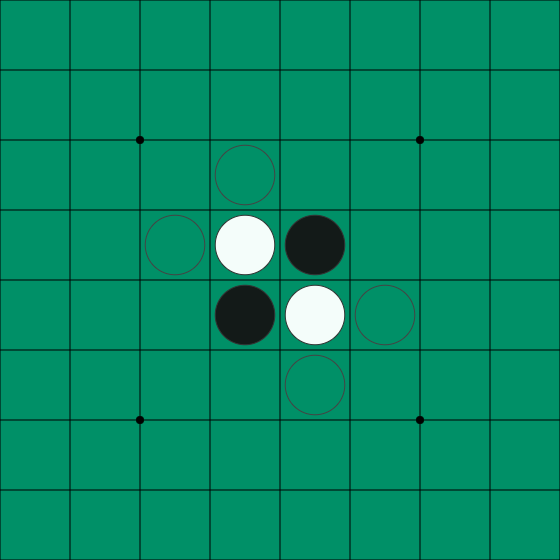
\includegraphics[width=0.7\textwidth]{ressources/plateau_init.png}
    \caption{Configuration initiale du plateau de jeu. Source : \href{https://www.eothello.com/}{eOthello}.}
    \label{fig:init_board}
\end{figure}

Elle s'encode comme suit. '0b', '0x' indiquent respectivement un nombre binaire et hexadécimal ; les underscores sont là pour faciliter la lecture :
\newline \newline
\noindent Le plateau noir : 
\begin{align*}
0b00000000\_00000000\_00000000\_00001000\_00010000\_00000000\_00000000\_00000000 \\
\end{align*}
Le plateau blanc :
\begin{align*}
0b00000000\_00000000\_00000000\_00010000\_00001000\_00000000\_00000000\_00000000 \\
\end{align*}
Ces deux entiers peuvent être réécris en hexadécimal pour une meilleure lisibilité :
\begin{align*}
    &0x00\_00\_00\_08\_10\_00\_00\_00 \quad (noir)\\
    &0x00\_00\_00\_10\_08\_00\_00\_00 \quad (blanc)\\
\end{align*}

Il est possible de récupérer la valeur d'une case $c_{i,j}$ d'un bitboard $b$ en utilisant la formule suivante : 
\begin{align*}
    (b\quad \gg\quad (8\times i+j))\quad \&\quad 1
\end{align*}
Avec $i$ la ligne, $j$ la colonne, $\gg$ l'opérateur de décalage à droite, et $\&$ l'opérateur logique 'et'.

Similairement, nous pouvons définir une case $c_{i,j}$ d'un bitboard $b$ en utilisant la formule suivante :
\begin{align*}
    b\quad |\quad (1\quad \ll\quad (8\times i+j))
\end{align*}
Avec $\ll$ l'opérateur de décalage à gauche, et $|$ l'opérateur logique 'ou'.

Nous obtenons toutes les pièces posées et toutes les cases vides avec les opérations logiques suivantes :
\begin{align*}
    &\text{pieces} = \text{noir} \quad | \quad \text{blanc} \\
    &\text{vides} = \sim \text{pieces}
\end{align*}
Avec $\sim$ l'opérateur logique 'non'.

De manière générale, n'importe quel pion ou coup peut être ajouté au plateau avec l'opérateur logique 'ou'.


\section{Algorithmes}
\label{sec:algo}

\subsubsection{Comment décaler un bitboard ?}
\label{subsec:shift}
Le calcul des coups valides est une étape cruciale pour le jeu, c'est par ailleurs l'étape la plus couteuse en temps de calcul. La représentation en bitboards nous permet de calculer les coups valides de manière très efficace, en vectorisant les opérations. Il est en effet possible de calculer simultanément les coups valides qui sont dans la même direction, en utilisant des masques prédéfinis. 

Pour cela, il va nous falloir être capable de décaler un plateau entier dans les 8 directions cardinales. Nous le faisons en utilisant des opérations logiques, comme le montre le pseudo-code ci-après.
\begin{algorithm}
    \caption{Opérations de décalage pour les coups valides.}
    \begin{algorithmic}[1]
    \Function{Nord}{$x$}
        \State \Return $x \gg 8$
    \EndFunction
    
    \Function{Sud}{$x$}
        \State \Return $(x \,\, \& \,\, 0x00ffffffffffffff) \ll 8$
    \EndFunction
    
    \Function{Est}{$x$}
        \State \Return $(x \,\, \& \,\, 0x7f7f7f7f7f7f7f7f) \ll 1$
    \EndFunction
    
    \Function{Ouest}{$x$}
        \State \Return $(x \,\, \& \,\, 0xfefefefefefefefe) \gg 1$
    \EndFunction
    \end{algorithmic}
    \label{alg:shift_ops}
\end{algorithm}

Les masques permettent d'éviter un débordement ou \textit{overflow}, une sortie de plateau, et de préserver les bords. Ils consistent à mettre à 0 les bits qui sont des positions sensibles dans la direction donnée. Nous obtenons ensuite $Nord-Est$, $Nord-Ouest$, $Sud-Est$, $Sud-Ouest$ en combinant les opérations précédentes. (Voir appendix \ref{app:logical_ops} pour plus de détails, ainsi que les codes python correspondant).

\subsection{Trouver les coups valides}
\label{subsec:valid_moves}

\subsection{Jouer un coup}
\label{subsec:play}


\newpage

\chapter{Validation}
\label{ch:validation}
Nous désirons mesurer deux aspects de notre programme : la qualité des stratégies décrites dans le sujet de \ac{TP} et la complexité de chaque algorithme. Pour cela, nous avons mis en place un championnat qui oppose différentes configurations, ainsi que des mesures de complexité pour chaque algorithme. Les statistiques sont obtenues sur 100 itérations, sauf pour certaines profondeurs 6 pour des raisons de temps de calcul. Les résultats sont présentés dans les sections suivantes.


\section{Mesure de complexité : Exploration de l'arbre de jeu}
\label{sec:game_tree_exploration}
Nous comparons ici la complexité en temps et en nombre de nœuds explorés. Nous avons mesuré ces deux aspects sur 24 configurations. Elles correspondent à un affrontement entre soit Minimax, soit Alpha-Beta contre un joueur aléatoire avec une profondeur de recherche de 2, 4 et 6, sur différentes stratégies.


\begin{table}[H]
    \centering
    \caption{NegamaxAlphaBeta/Negamax Analyse comparative du temps d'exécution d'une partie à travers les profondeurs et les stratégies en secondes}
    \resizebox{0.85\textwidth}{!}{% Resize table to fit within the text width, keeping aspect ratio
        \begin{tabular}{
            @{}
            >{\raggedright\arraybackslash}p{1cm}
            >{\raggedright\arraybackslash}p{4cm}
            S
            S
            S
            @{}
            }
            \toprule
            \textbf{Depth} & \textbf{Strategy}           & {\textbf{Mean}}             & {\textbf{Std}}             \\
            \midrule
            \multicolumn{4}{c}{\textbf{Depth 2}}                                                                    \\
            \midrule
                           & Positional                  & {74.10\% (0.03 vs 0.04)}    & {198.71\% (0.02 vs 0.01)}  \\
                           & Absolute                    & {86.94\% (0.01 vs 0.02)}    & {208.26\% (0.02 vs 0.01)}  \\
                           & Mobility                    & {54.55\% (0.06 vs 0.12)}    & {83.37\% (0.02 vs 0.03)}   \\
                           & Mixed (thresholds=[30, 55]) & {67.22\% (0.06 vs 0.08)}    & {140.54\% (0.04 vs 0.03)}  \\
            \midrule
            \multicolumn{4}{c}{\textbf{Depth 4}}                                                                    \\
            \midrule
                           & Positional                  & {14.56\% (0.90 vs 6.21)}    & {14.38\% (0.30 vs 2.06)}   \\
                           & Absolute                    & {24.09\% (0.51 vs 2.10)}    & {16.92\% (0.19 vs 1.15)}   \\
                           & Mobility                    & {13.04\% (1.50 vs 11.52)}   & {11.27\% (0.49 vs 4.38)}   \\
                           & Mixed (thresholds=[30, 55]) & {15.93\% (1.17 vs 7.34)}    & {12.67\% (0.40 vs 3.18)}   \\
            \midrule
            \multicolumn{4}{c}{\textbf{Depth 6}}                                                                    \\
            \midrule
                           & Positional                  & {8.45\% (35.20 vs 416.65)}  & {2.60\% (2.82 vs 108.49)}  \\
                           & Absolute                    & {12.23\% (20.14 vs 164.64)} & {18.39\% (13.95 vs 75.87)} \\
                           & Mobility                    & {2.83\% (39.32 vs 1390.49)} & {1.03\% (7.65 vs 745.69)}  \\
                           & Mixed (thresholds=[30, 55]) & {3.17\% (17.34 vs 546.98)}  & {4.36\% (5.04 vs 115.61)}  \\
            \bottomrule
        \end{tabular}
    }
\end{table}

L'unité est la seconde. Nous avons mesuré le temps de calcul pour chaque partie jouée.


\subsection{Nombre de nœuds explorés}
\label{subsec:node_explored}
Nous avons mesuré à chaque coup des joeurs, le nombre de nœuds explorés. Nous pouvons donc comparer chaque algorithme sur un graphe pour chaque profondeur donnée\footnote{Chaque figure est disponible séparément dans les appendices \ref{app:node_explored}.}. Nous avons également calculé le nombre moyen de nœuds explorés pour chaque configuration. Les résultats sont présentés dans les tableaux \ref{tab:node_explored_summary} et \ref{tab:node_explored_summary-2}.

\begin{figure}[H]
    \centering
    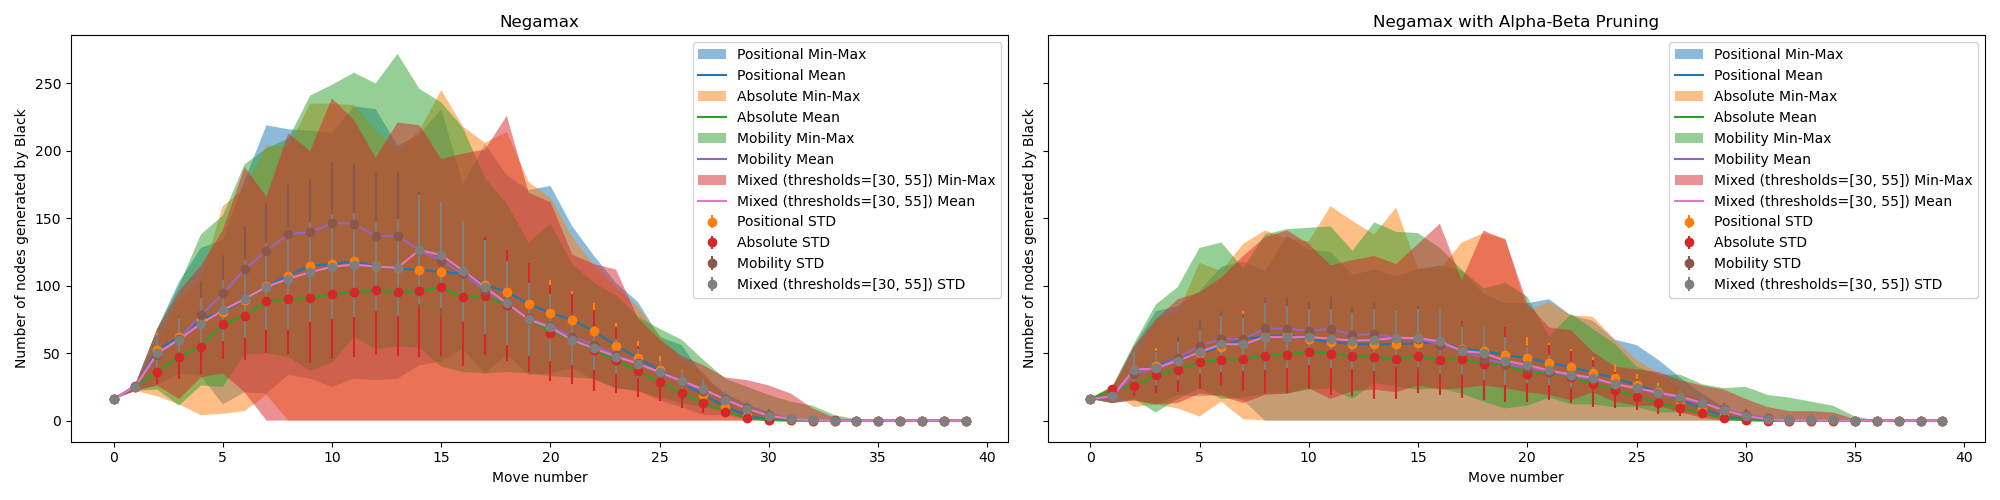
\includegraphics[width=\textwidth]{ressources/Number of nodes generated by Black_depth_2_combined.png}
    \caption{Nombre de nœuds explorés par Minimax et Alpha-Beta en profondeur 2.}
    \label{fig:complexity_node_explored-2}
\end{figure}

\begin{figure}[H]
    \centering
    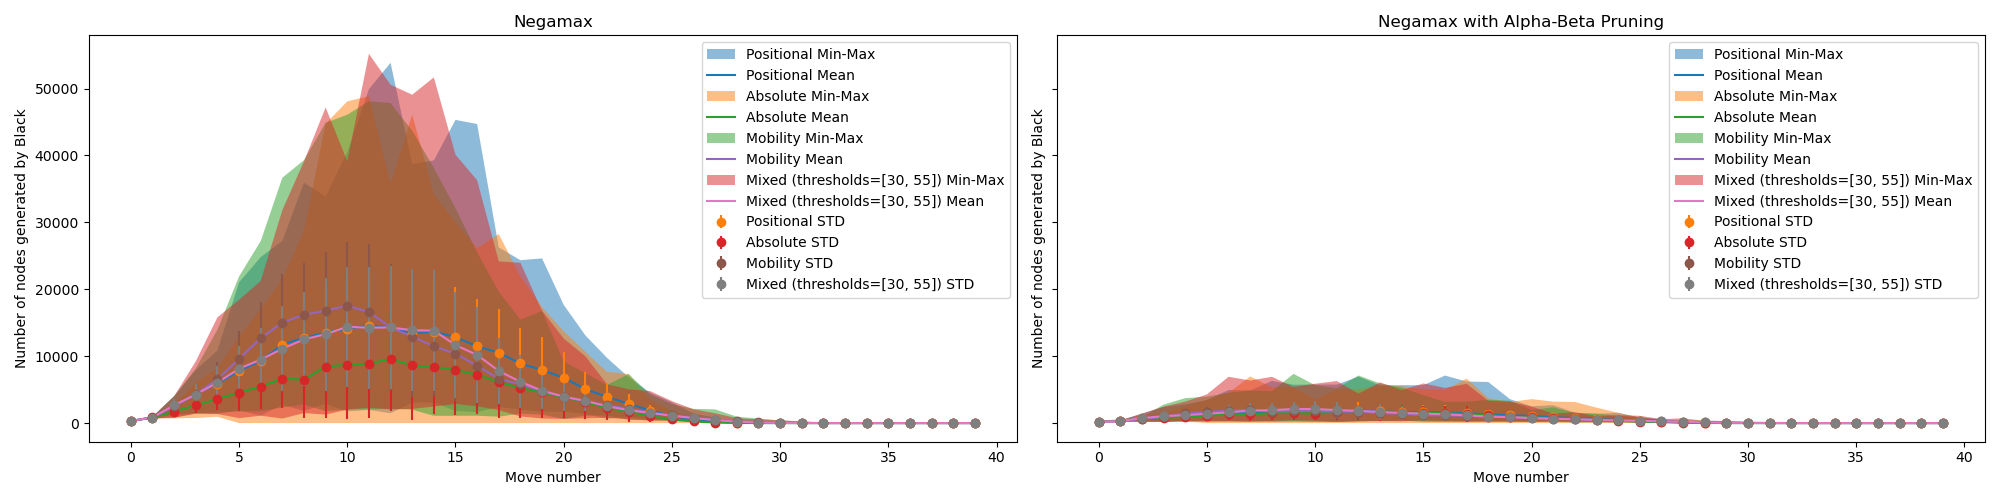
\includegraphics[width=\textwidth]{ressources/Number of nodes generated by Black_depth_4_combined.png}
    \caption{Nombre de nœuds explorés par Minimax et Alpha-Beta en profondeur 4.}
    \label{fig:complexity_node_explored-4}
\end{figure}

\begin{figure}[H]
    \centering
    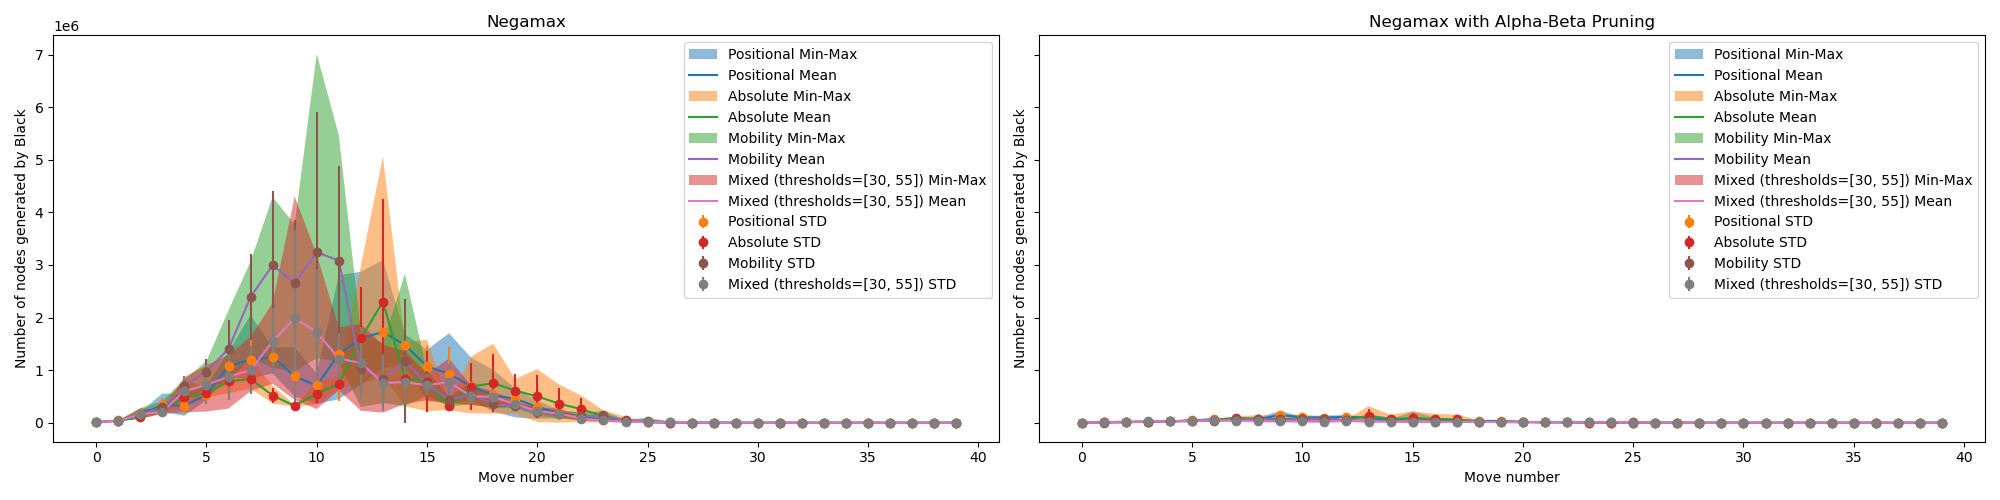
\includegraphics[width=\textwidth]{ressources/Number of nodes generated by Black_depth_6_combined.png}
    \caption{Nombre de nœuds explorés par Minimax et Alpha-Beta en profondeur 6.}
    \label{fig:complexity_node_explored-6}
\end{figure}

Dans un tableau récapitulatif, nous pouvons observer le nombre moyen de nœuds explorés par Minimax et Alpha-Beta pour chaque profondeur. Les résultats sont présentés dans le tableau \ref{tab:node_explored_summary}. Pour les valeurs exactes, voir le tableau \ref{tab:node_explored_summary-2}, avec pour unité $10^4$ le nombre de nœuds explorés.

\begin{table}[H]
    \centering
    \caption{NegamaxAlphaBeta (gauche)/Negamax(droite) Analyse comparative du nombre de nœuds explorés à travers les profondeurs et les stratégies en pourcentage}
    \resizebox{\textwidth}{!}{% Resize table to fit within the text width, keeping aspect ratio
        \begin{tabular}{
            @{}
            >{\raggedright\arraybackslash}p{1cm}
            >{\raggedright\arraybackslash}p{4cm}
            S
            S
            S
            @{}
            }
            \toprule
            \textbf{Depth} & \textbf{Strategy}           & {\textbf{Max of Maxs}} & {\textbf{Mean of Means}} & {\textbf{Mean of Stds}} \\
            \midrule
            \multicolumn{5}{c}{\textbf{Depth 2}}                                                                                       \\
            \cmidrule(lr){1-5}
                           & Positional                  & 58.80\%                & 57.52\%                  & 65.20\%                 \\
                           & Absolute                    & 64.90\%                & 55.79\%                  & 63.92\%                 \\
                           & Mobility                    & 54.04\%                & 53.95\%                  & 60.26\%                 \\
                           & Mixed (thresholds=[30, 55]) & 61.09\%                & 58.35\%                  & 62.72\%                 \\
            \midrule
            \multicolumn{5}{c}{\textbf{Depth 4}}                                                                                       \\
            \cmidrule(lr){1-5}
                           & Positional                  & 13.19\%                & 14.77\%                  & 16.35\%                 \\
                           & Absolute                    & 14.27\%                & 21.19\%                  & 17.92\%                 \\
                           & Mobility                    & 15.29\%                & 14.06\%                  & 14.30\%                 \\
                           & Mixed (thresholds=[30, 55]) & 12.54\%                & 15.76\%                  & 15.56\%                 \\
            \midrule
            \multicolumn{5}{c}{\textbf{Depth 6}}                                                                                       \\
            \cmidrule(lr){1-5}
                           & Positional                  & 7.15\%                 & 6.96\%                   & 6.66\%                  \\
                           & Absolute                    & 6.26\%                 & 7.67\%                   & 10.21\%                 \\
                           & Mobility                    & 1.93\%                 & 2.98\%                   & 2.56\%                  \\
                           & Mixed (thresholds=[30, 55]) & 1.84\%                 & 3.07\%                   & 2.77\%                  \\
            \bottomrule
        \end{tabular}
    }
    \label{tab:node_explored_summary}
\end{table}

\begin{table}[H]
    \centering
    \caption{NegamaxAlphaBeta (gauche)/Negamax(droite) Analyse comparative du nombre de nœuds explorés à travers les profondeurs et les stratégies en valeur exacte}
    \resizebox{\textwidth}{!}{% Resize table to fit within the text width, keeping aspect ratio
        \begin{tabular}{
            @{}
            >{\raggedright\arraybackslash}p{1cm}
            >{\raggedright\arraybackslash}p{4cm}
            S
            S
            S
            @{}
            }
            \toprule
            \textbf{Depth} & \textbf{Strategy}           & {\textbf{Max of Maxs}} & {\textbf{Mean of Means}} & {\textbf{Mean of Stds}} \\
            \midrule
            \multicolumn{5}{c}{\textbf{Depth 2}}                                                                                       \\
            \cmidrule(lr){1-5}
                           & Positional                  & {0.0137 vs 0.0233}     & {0.003193 vs 0.005551}   & {0.001091 vs 0.001673}  \\
                           & Absolute                    & {0.0159 vs 0.0245}     & {0.002579 vs 0.004622}   & {0.001411 vs 0.002208}  \\
                           & Mobility                    & {0.0147 vs 0.0272}     & {0.003256 vs 0.006036}   & {0.001102 vs 0.001830}  \\
                           & Mixed (thresholds=[30, 55]) & {0.0146 vs 0.0239}     & {0.003178 vs 0.005445}   & {0.001087 vs 0.001734}  \\
            \midrule
            \multicolumn{5}{c}{\textbf{Depth 4}}                                                                                       \\
            \cmidrule(lr){1-5}
                           & Positional                  & {0.7103 vs 5.3861}     & {0.078708 vs 0.532977}   & {0.046724 vs 0.285685}  \\
                           & Absolute                    & {0.6975 vs 4.8871}     & {0.068316 vs 0.3224}     & {0.046545 vs 0.259710}  \\
                           & Mobility                    & {0.7352 vs 4.8096}     & {0.073940 vs 0.525755}   & {0.040591 vs 0.283905}  \\
                           & Mixed (thresholds=[30, 55]) & {0.6921 vs 5.5201}     & {0.077103 vs 0.489311}   & {0.044621 vs 0.286737}  \\
            \midrule
            \multicolumn{5}{c}{\textbf{Depth 6}}                                                                                       \\
            \cmidrule(lr){1-5}
                           & Positional                  & {22.08 vs 309.04}      & {2.96 vs 42.50}          & {1.13 vs 16.93}         \\
                           & Absolute                    & {31.68 vs 506.37}      & {2.77 vs 36.06}          & {1.98 vs 19.34}         \\
                           & Mobility                    & {13.56 vs 701.55}      & {1.79 vs 60.19}          & {0.779 vs 30.44}        \\
                           & Mixed (thresholds=[30, 55]) & {7.90 vs 430.26}       & {1.24 vs 40.39}          & {0.582 vs 20.99}        \\
            \bottomrule
        \end{tabular}
    }
    \label{tab:node_explored_summary-2}
\end{table}



\section{Championnat : Comparaison des algorithmes}
\label{sec:championship}


\newpage

\section{Discussion}
\label{sec:discussion}
\newpage

\chapter{Conclusion}
\label{chap:conclusion}

Ce projet a permis d'explorer en profondeur les mécanismes des algorithmes min-max et Alpha-Beta dans le contexte du jeu d'Othello, un environnement aux règles simples mais à la complexité combinatoire élevée. Nous avons développé et évalué plusieurs stratégies d'intelligence artificielle, notamment les approches positionnelle, absolue, mobilité et mixte, en les faisant jouer les unes contre les autres ainsi que contre des joueurs humains. Nos résultats montrent que l'algorithme Alpha-Beta, en particulier, offre des avantages significatifs en termes de réduction de la complexité temporelle et de l'espace de recherche, ce qui le rend préférable pour des profondeurs de recherche élevées.

L'analyse de la performance des différents agents a révélé que les stratégies mixtes, qui adaptent leur approche selon la phase du jeu, étaient particulièrement efficaces, combinant les avantages des approches positionnelles, de mobilité et absolues au fur et à mesure que la partie progresse. Cela souligne l'importance d'une adaptation stratégique flexible en réponse à l'évolution de l'état du jeu. Aussi, les stratégies positionnelles, prédominantes dans Mixte, ne peuvent pas être négligées, car elles sont elle-même très efficaces. La connaissance préalable du jeu est donc un atout majeur pour l'IA.

Les défis rencontrés, notamment liées à la gestion de la complexité exponentielle et l'ordre d'exploration des nœuds, nous ont conduit à introduire plusieurs optimisations, telles que la représentation en BitBoard, un algorithme efficace de calcul des coups valides, et l'implémentation de l'élagage Alpha-Beta. Ces techniques ont permis de réduire considérablement le temps de calcul nécessaire pour explorer l'arbre de jeu, sans compromettre la qualité des décisions prises par l'IA.

D'autres améliorations futures sont envisageables, comme l'exploration de techniques de tri préalable des coups ou l'intégration de l'apprentissage par renforcement pour améliorer la capacité d'adaptation et d'apprentissage de l'IA. Il serait par ailleurs très intéressant de finir l'implémentation du modèle classifieur et de le comparer aux heuristiques existantes, ainsi qu'à l'état de l'art tel qu'Edax.

En conclusion, ce projet a non seulement renforcé notre compréhension des algorithmes de jeu à deux joueurs et de leurs applications pratiques mais a également ouvert la voie à de futures recherches sur l'optimisation des stratégies d'IA dans des jeux de complexité similaire. Nous avons pu démontrer que des avancées significatives sont possibles, même dans des contextes où les ressources de calcul sont limitées, par une utilisation judicieuse des techniques d'élagage et de l'analyse heuristique.

Sur un plan plus personnel, j'ai particulièrement aimé ce projet, et vais continuer à mettre à jour le dépôt github associé. J'espère pouvoir continuer à faire plus de Théorie des Jeux et surtout plus d'\ac{IA}, peut-être sur d'autres jeux de plateau. J'ai appris beaucoup de choses, et j'espère que ce rapport vous a plu. Merci de m'avoir lu.
\newpage

\appendix
\pagenumbering{Roman}
\renewcommand{\thepage}{\Roman{page}}

\chapter{Algorithmes et Code}

\section{Opérations Logiques}
\label{app:logical_ops}
En \ref{subsubsec:enc}, nous avons vu comment encoder en pseudo-code un pion et un plateau.
\\ \\
\noindent \textbf{En Python :}
\begin{figure}[H]
    \centering
    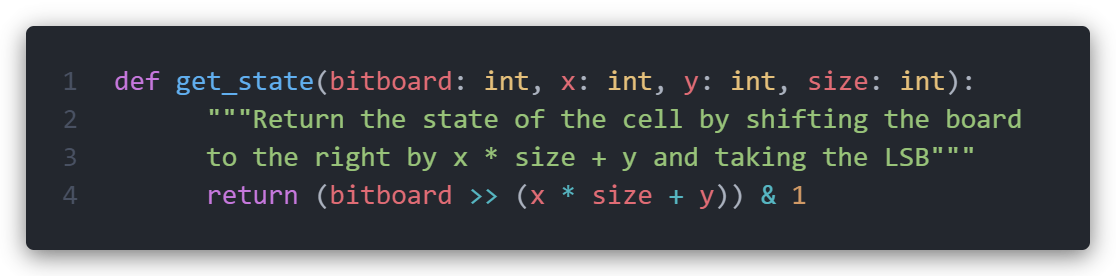
\includegraphics[width=1\textwidth]{ressources/get_state.png}
    \caption{Opérations logiques pour obtenir l'état du plateau.}
    \label{fig:get_state}
\end{figure}
\begin{figure}[H]
    \centering
    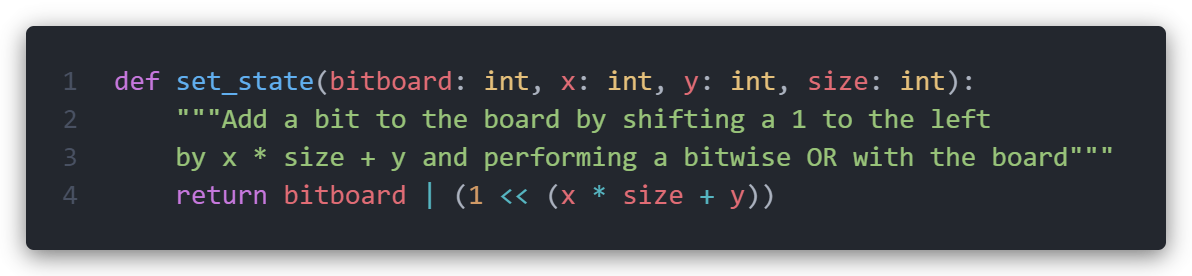
\includegraphics[width=1\textwidth]{ressources/set_state.png}
    \caption{Opérations logiques pour définir l'état du plateau.}
    \label{fig:set_state}
\end{figure}

En \ref{subsec:shift}, nous avons vu comment décaler un bitboard dans 4 directions cardinales. Voyons maintenant comment décaler un bitboard dans les 4 directions diagonales, et leur équivalent en python.

\begin{algorithm}[H]
    \caption{Opérations de décalage en diagonales.}
    \begin{algorithmic}[1]
    \Function{NordEst}{$x$}
        \State \Return $Nord(Est(x))$
    \EndFunction

    \Function{NordOuest}{$x$}
        \State \Return $Nord(Ouest(x))$
    \EndFunction

    \Function{SudEst}{$x$}
        \State \Return $Sud(Est(x))$
    \EndFunction

    \Function{SudOuest}{$x$}
        \State \Return $Sud(Ouest(x))$
    \EndFunction
    \end{algorithmic}
\end{algorithm}

\noindent \textbf{En Python :}
\begin{figure}[H]
    \centering
    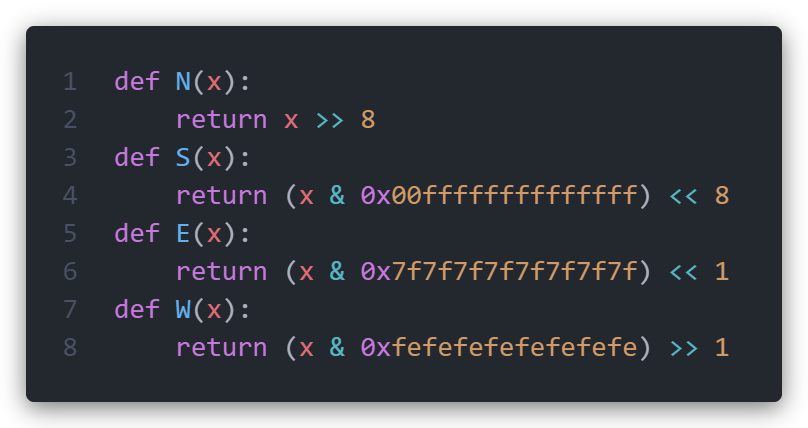
\includegraphics[width=0.8\textwidth]{ressources/operateurCardinaux.png}
    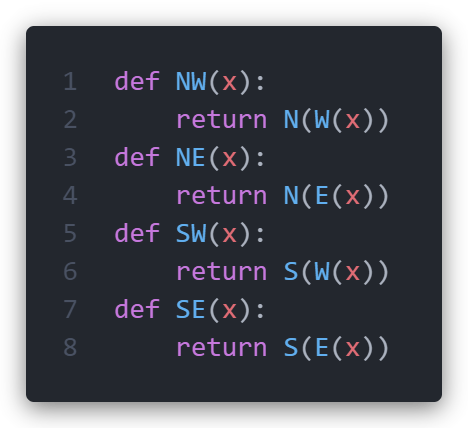
\includegraphics[width=0.5\textwidth]{ressources/operateurCardinauxComposes.png}
    \caption{Opérations de décalage pour les coups valides.}
    \label{fig:shift_ops}
\end{figure}

\section{Trouver et jouer coups valides}
\label{app:valid_moves}

En \ref{subsec:valid_moves}, nous avons vu comment trouver les coups valides et les jouer. Voyons maintenant en Python comment se traduit les pseudo-codes.

\begin{figure}[H]
    \centering
    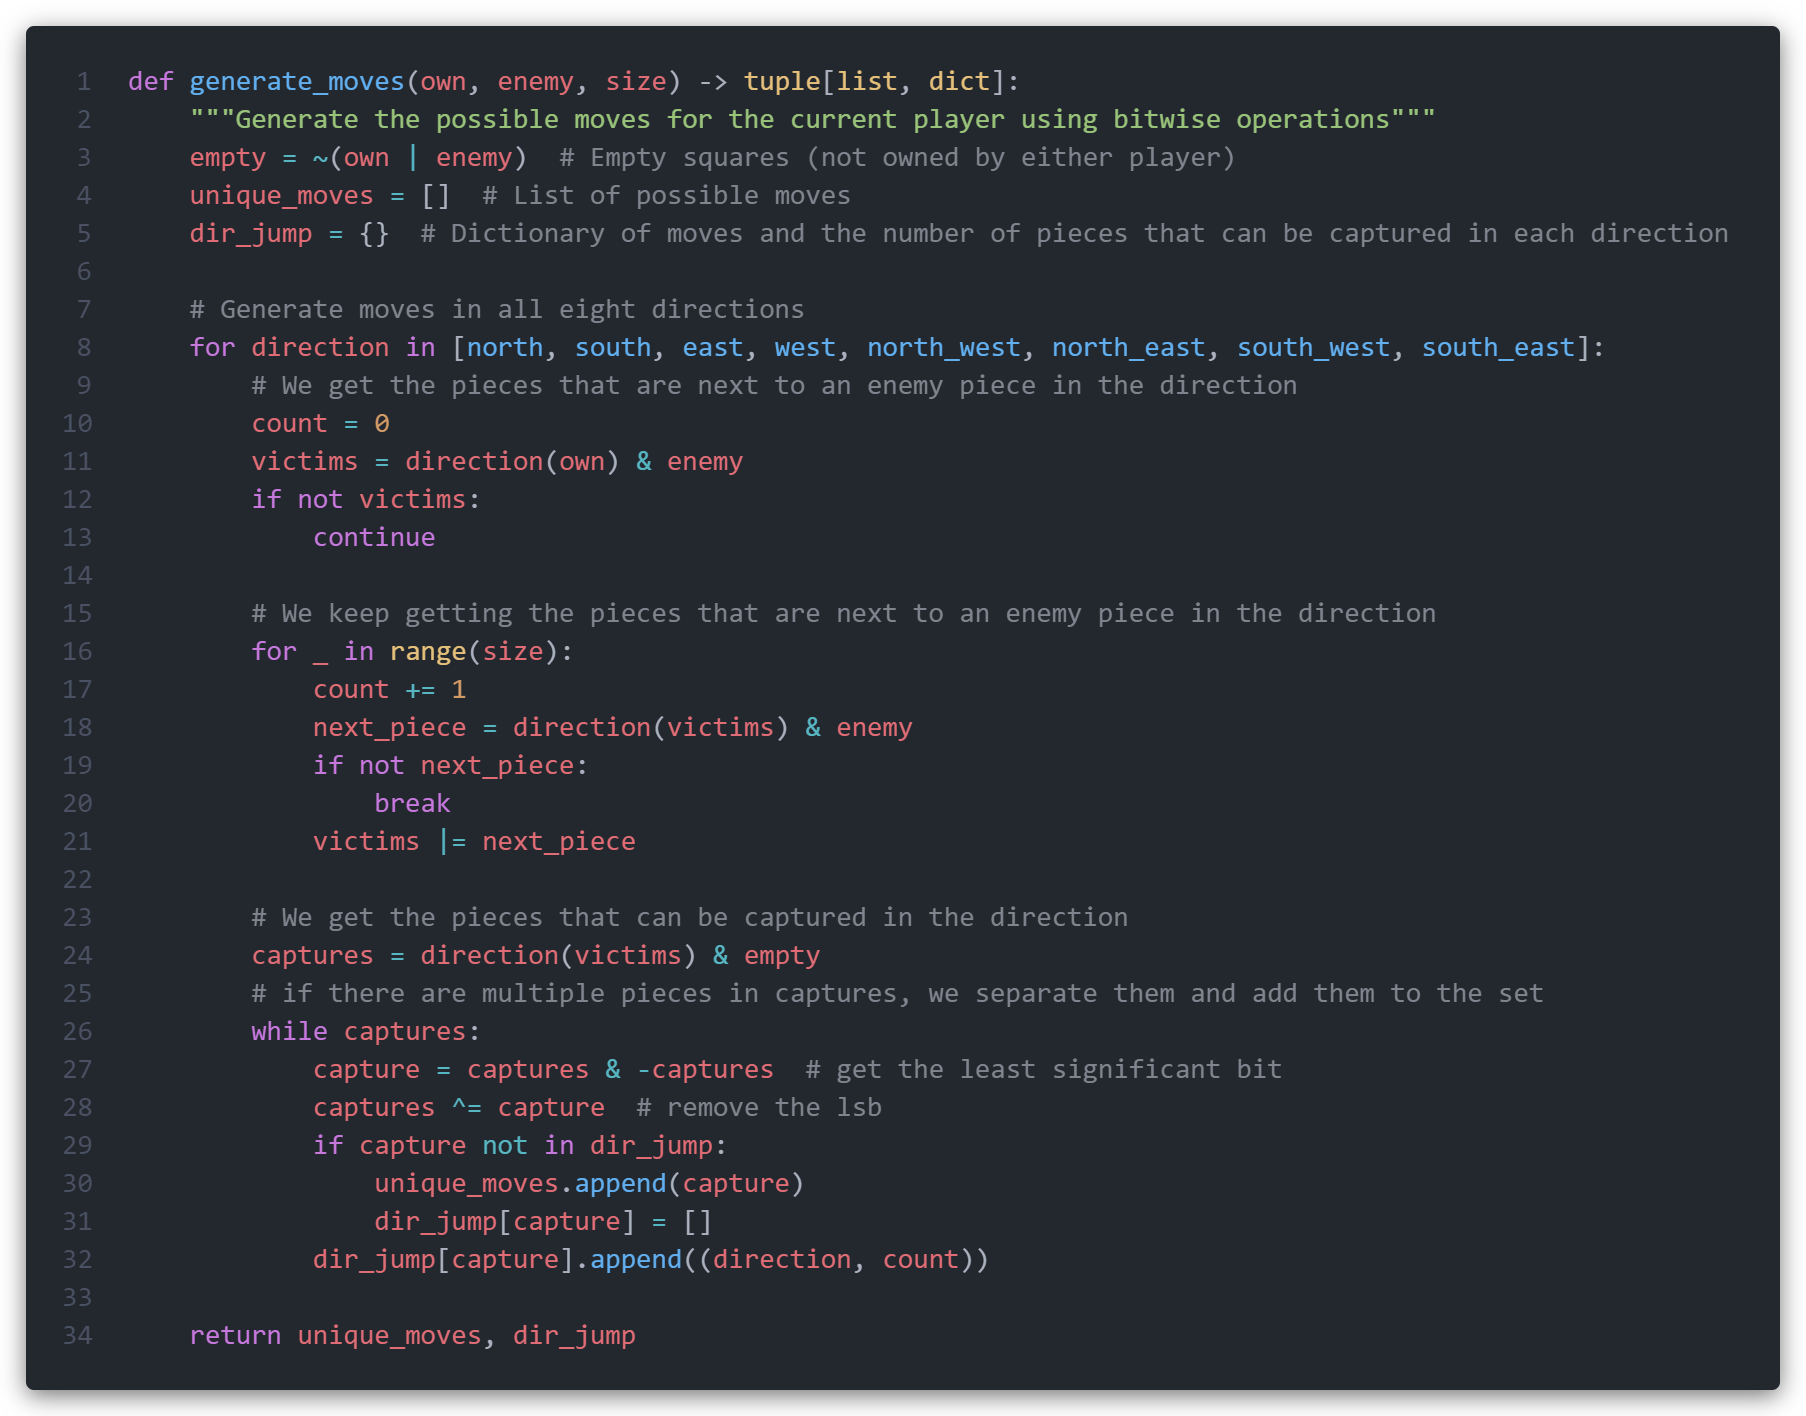
\includegraphics[width=1\textwidth]{ressources/generate_moves.png}
    \caption{Trouver les coups valides.}
    \label{fig:generate_moves}
\end{figure}

\begin{figure}[H]
    \centering
    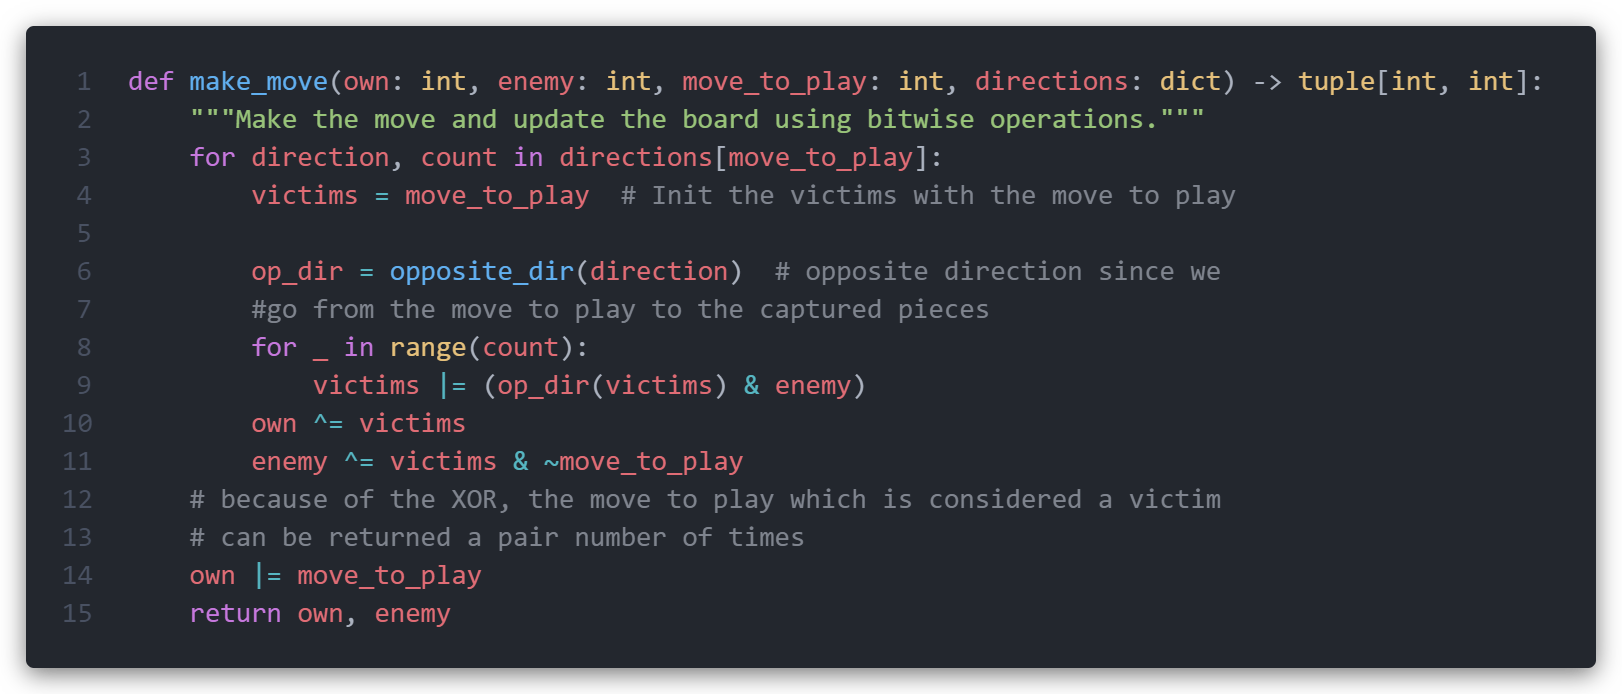
\includegraphics[width=1\textwidth]{ressources/make_move.png}
    \caption{Jouer un coup.}
    \label{fig:make_move}
\end{figure}

\section{Minimax}
\label{app:minimax}

En \ref{subsec:minimax}, nous avons vu comment implémenter l'algorithme Negamax avec AlphaBeta. Voyons maintenant en Python comment se traduit le pseudo-code, et les autres versions de l'algorithme.

\begin{figure}[H]
    \centering
    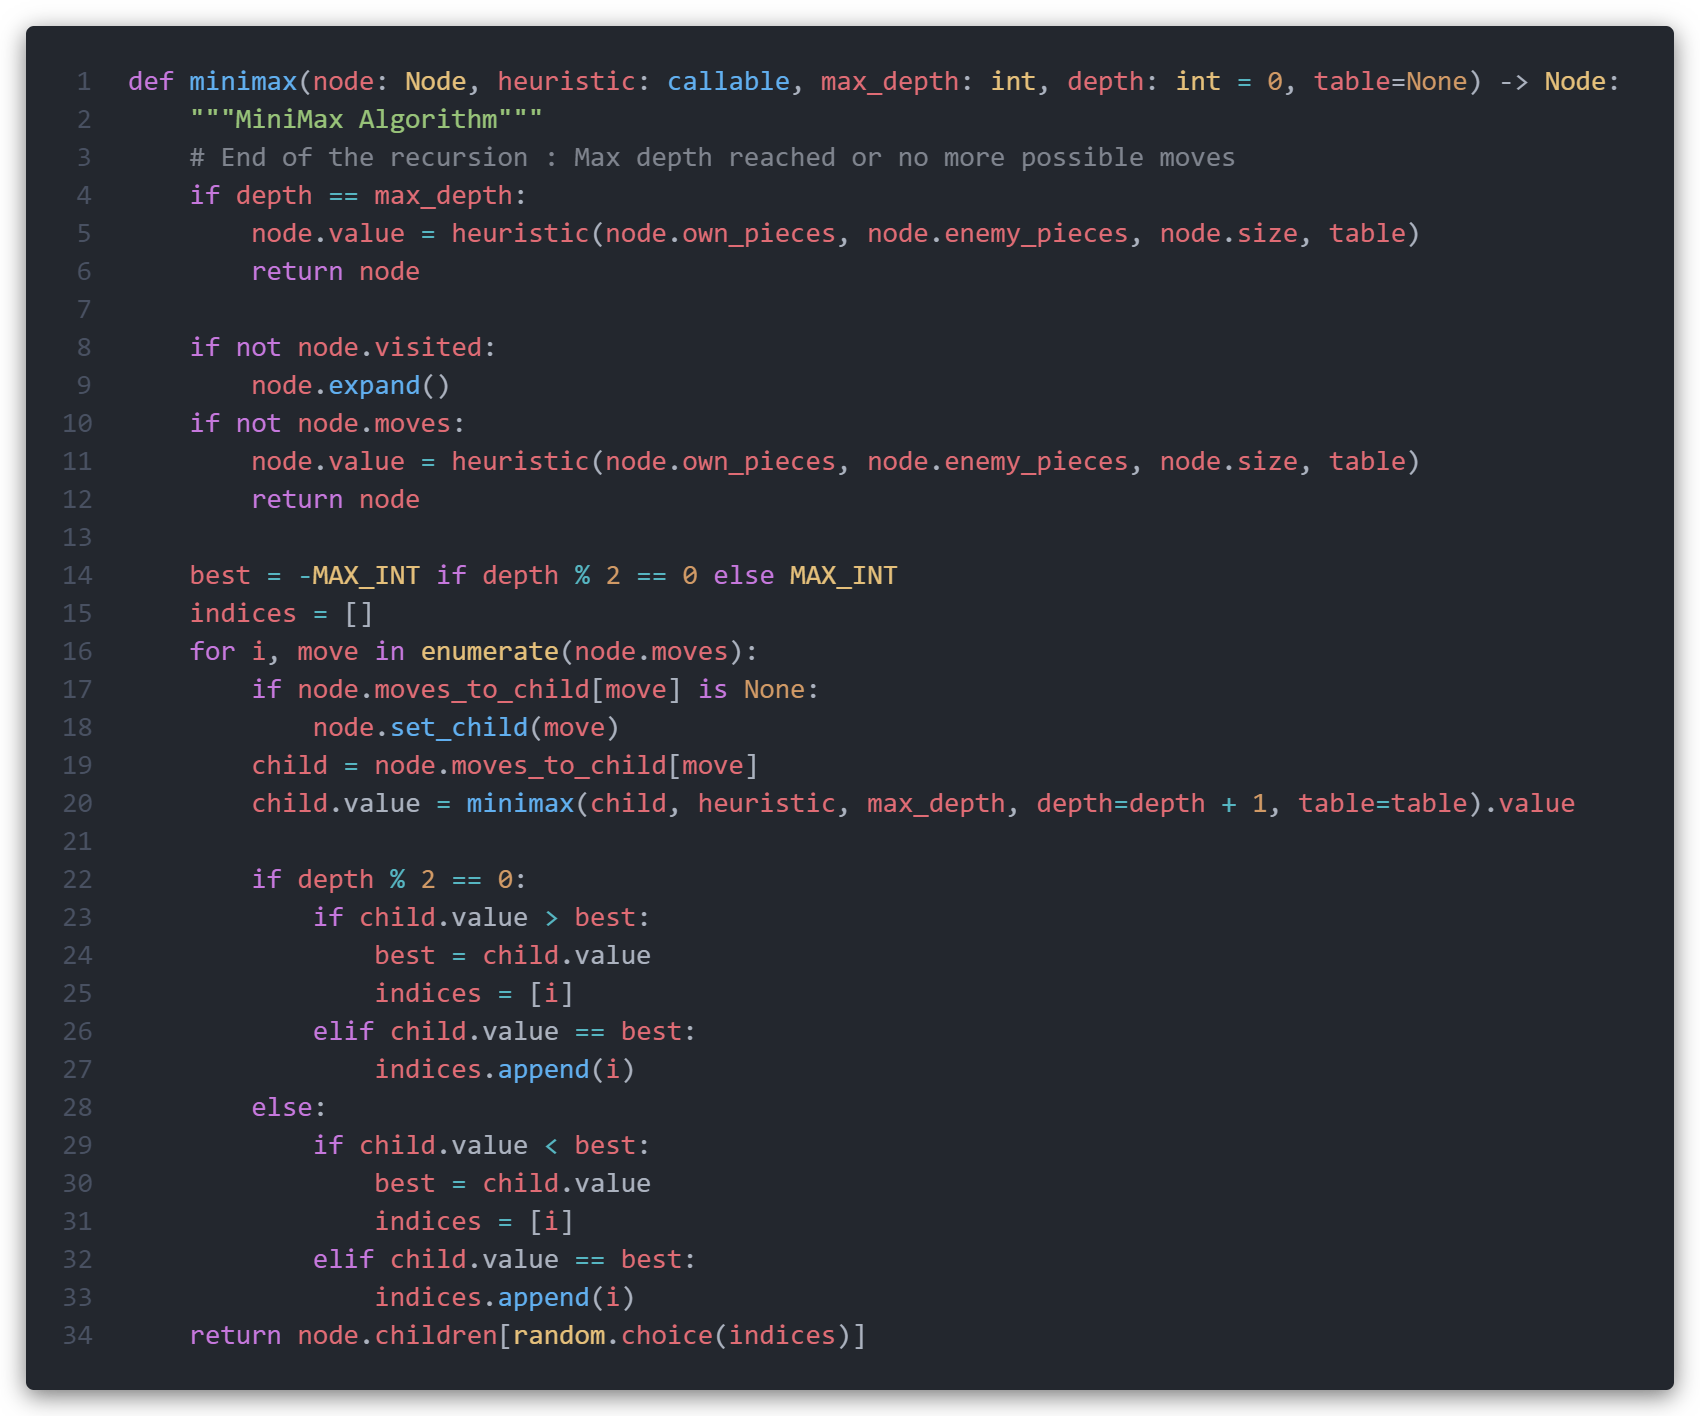
\includegraphics[width=1\textwidth]{ressources/minimax.png}
    \caption{Algorithme Minimax.}
    \label{fig:minimax}
\end{figure}

\begin{figure}[H]
    \centering
    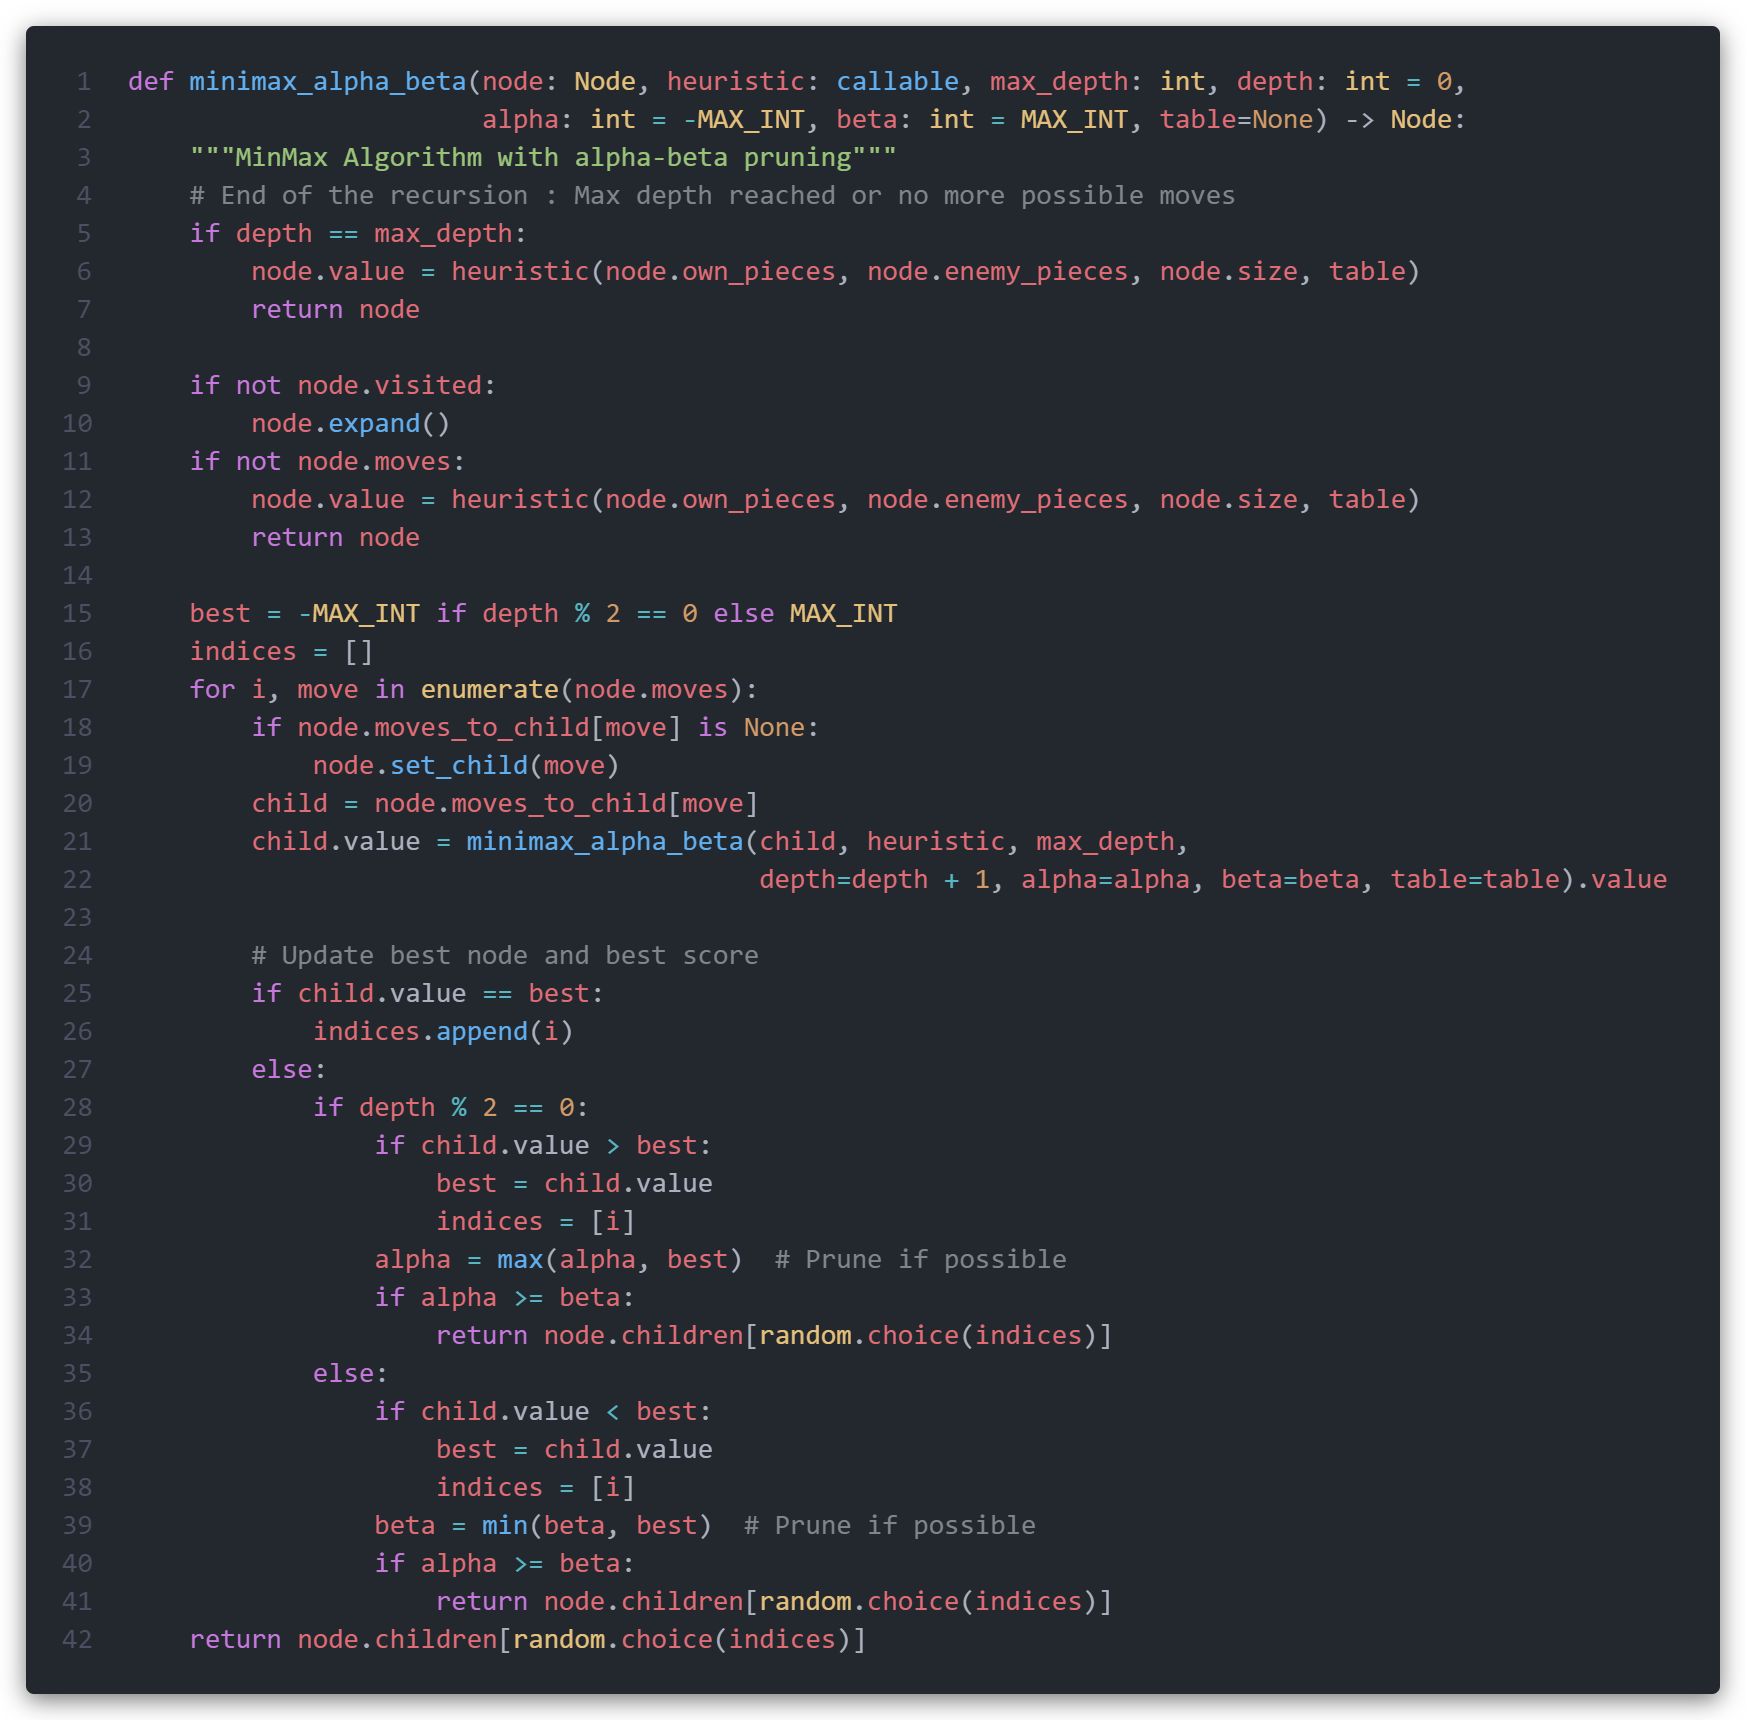
\includegraphics[width=1\textwidth]{ressources/minimax-a-b.png}
    \caption{Algorithme Minimax avec AlphaBeta.}
    \label{fig:minimax-a-b}
\end{figure}

\begin{figure}[H]
    \centering
    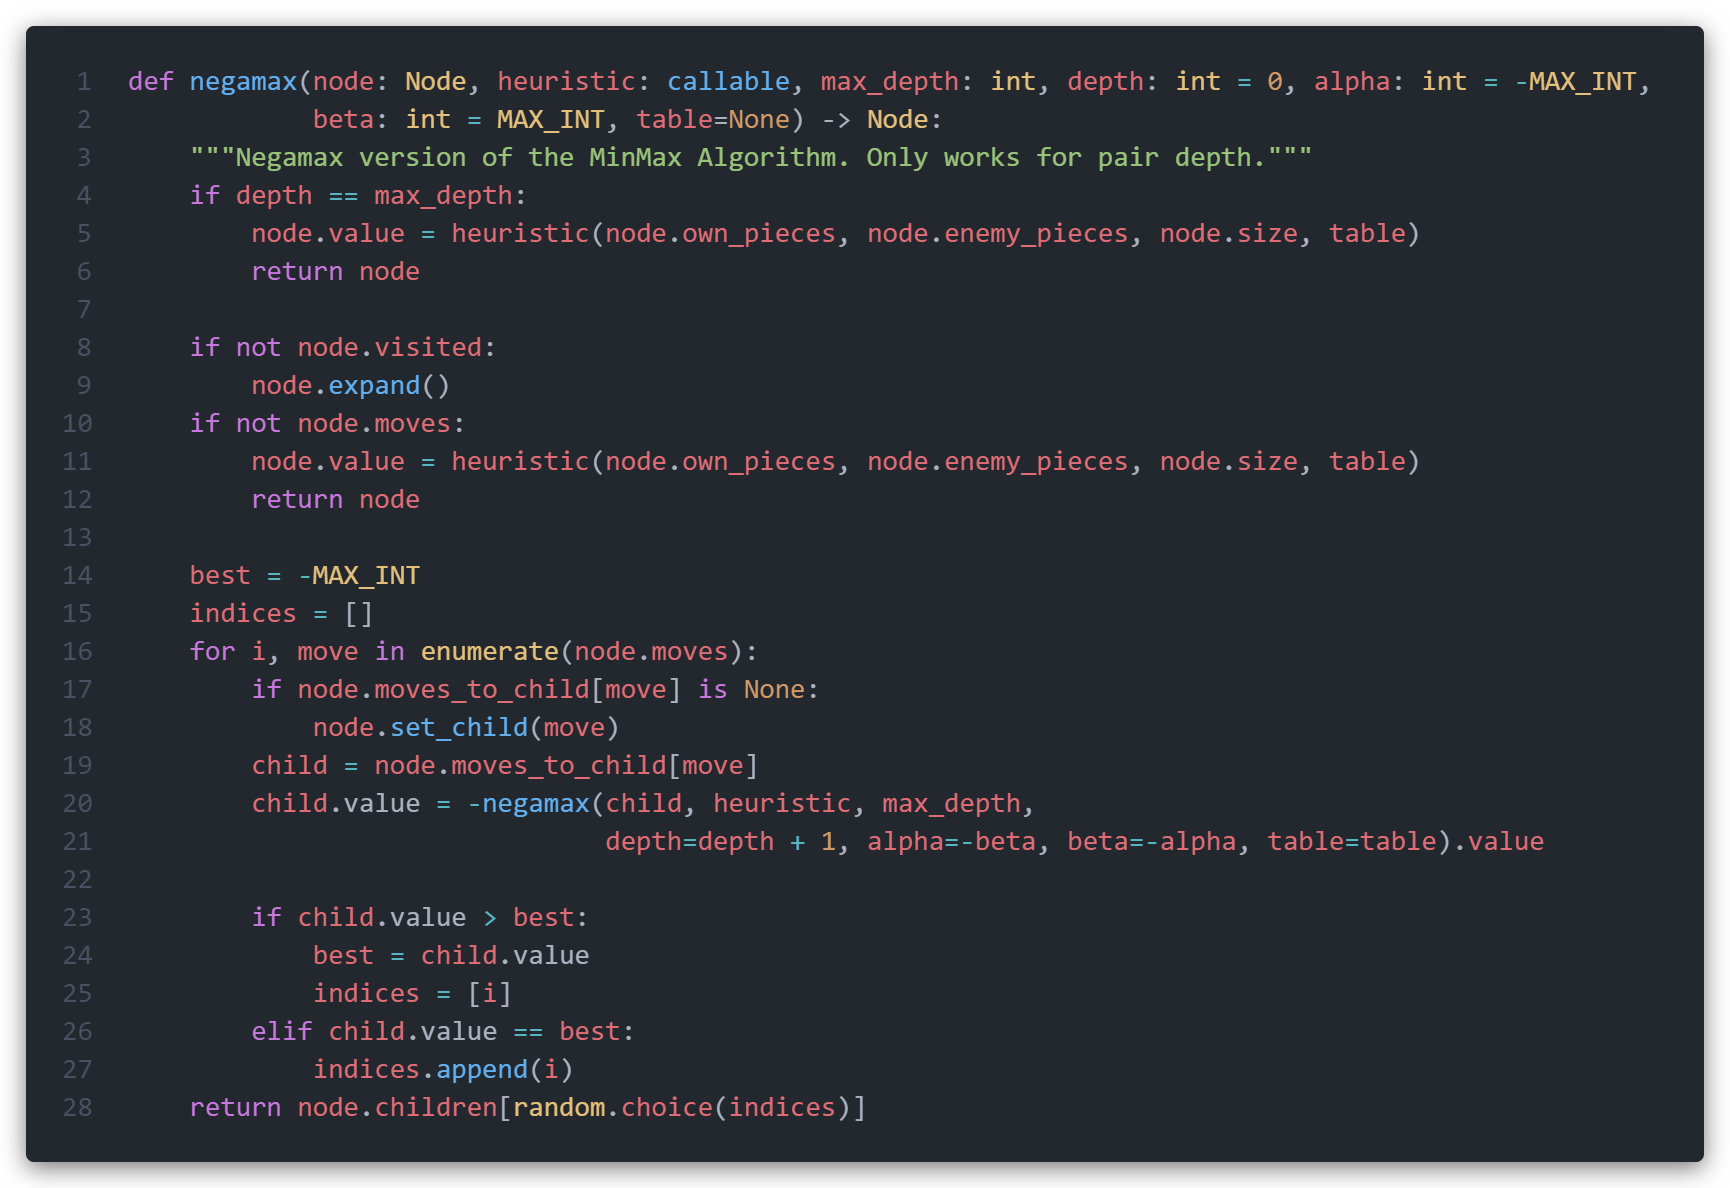
\includegraphics[width=1\textwidth]{ressources/negamax.png}
    \caption{Algorithme Negamax.}
    \label{fig:negamax}
\end{figure}


\begin{figure}[H]
    \centering
    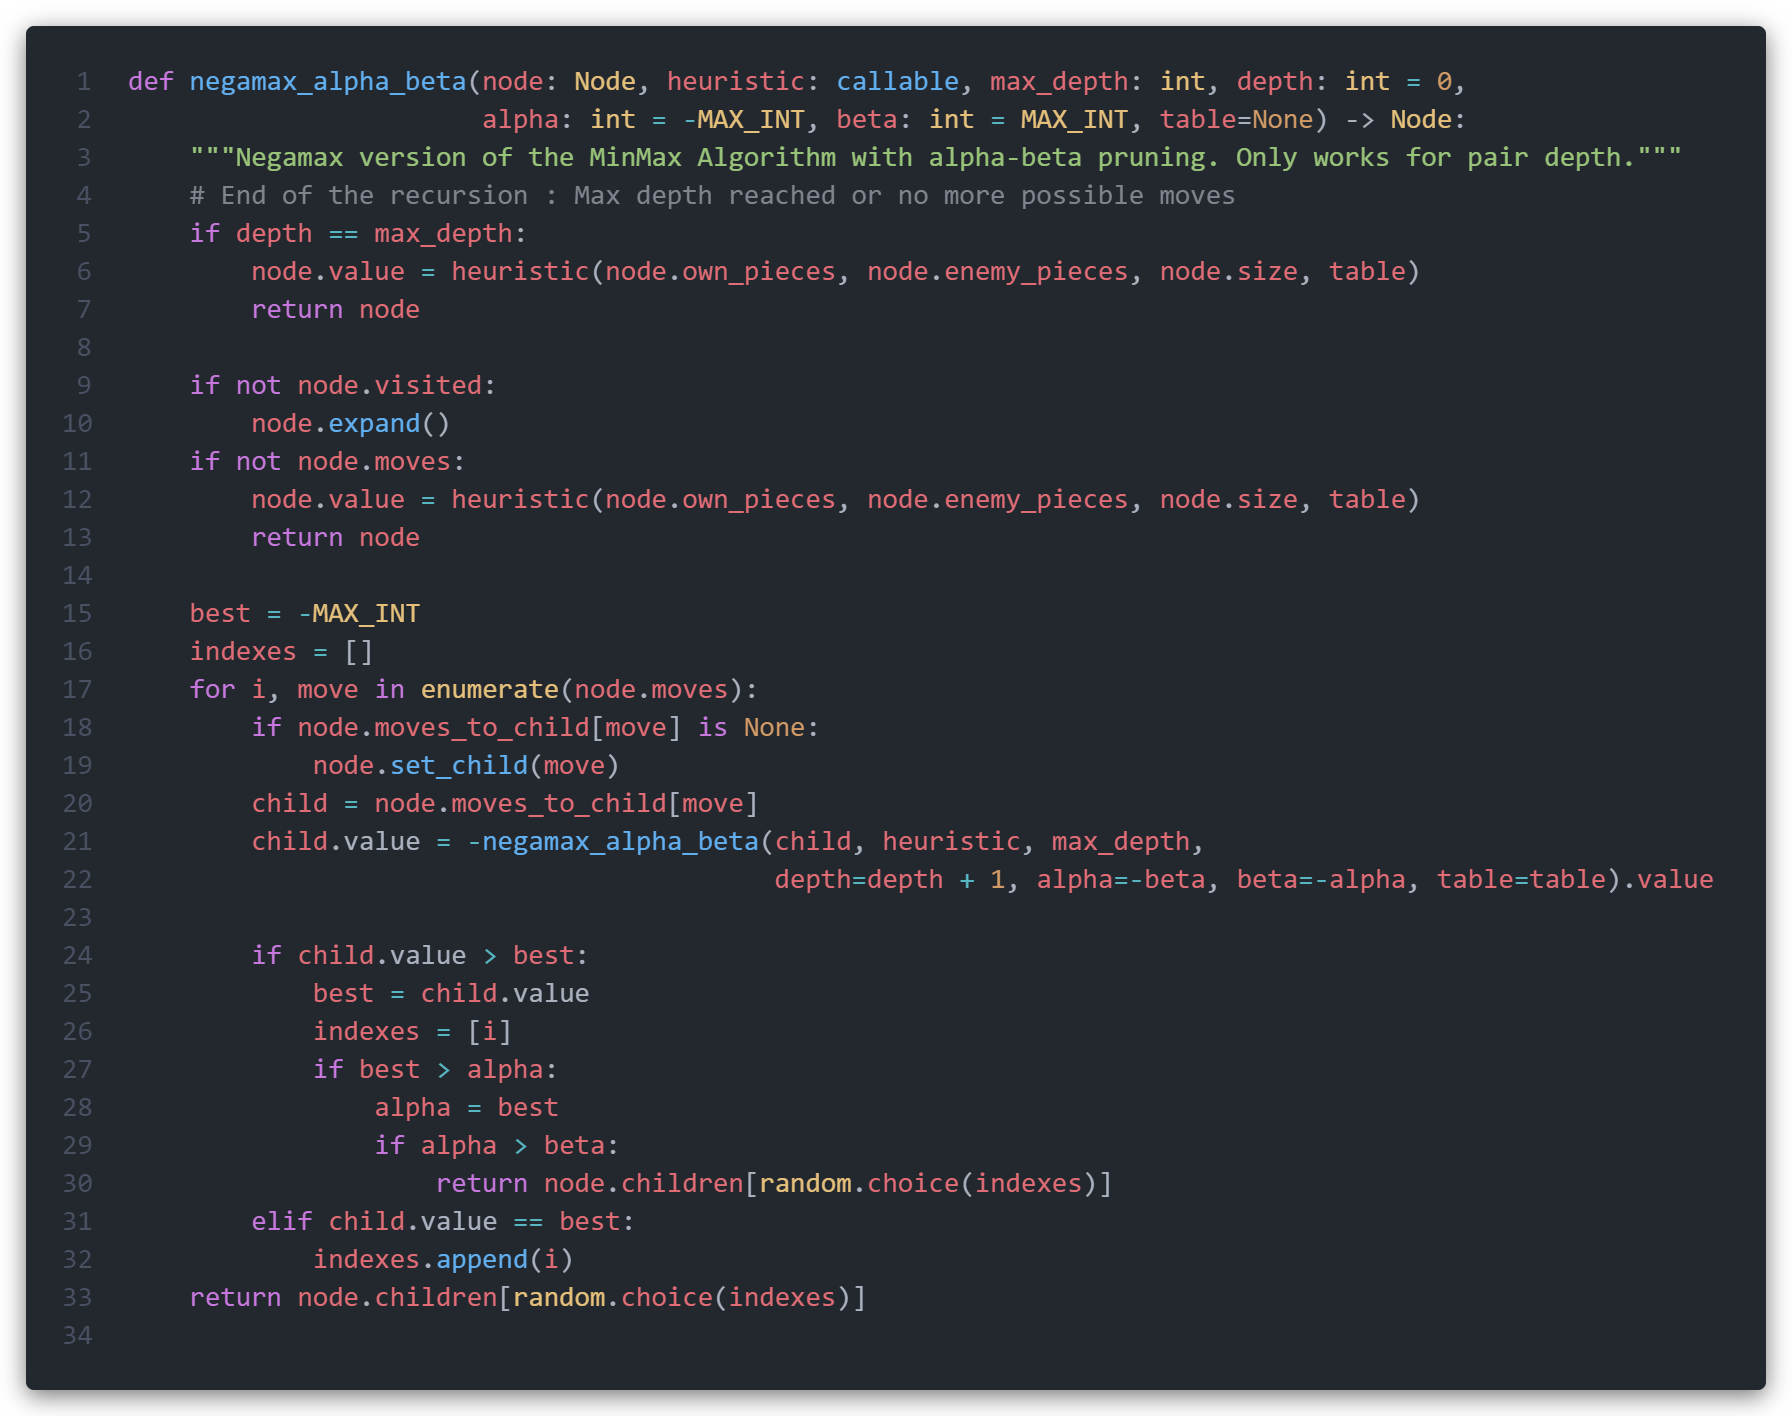
\includegraphics[width=1\textwidth]{ressources/nega-a-b.png}
    \caption{Algorithme Negamax avec AlphaBeta.}
    \label{fig:negamax-a-b}
\end{figure}


\chapter{Résultats et statistiques}
\section{Graphiques individuels des noeuds explorés}
\label{app:node_explored}

\begin{figure}[H]
    \centering
    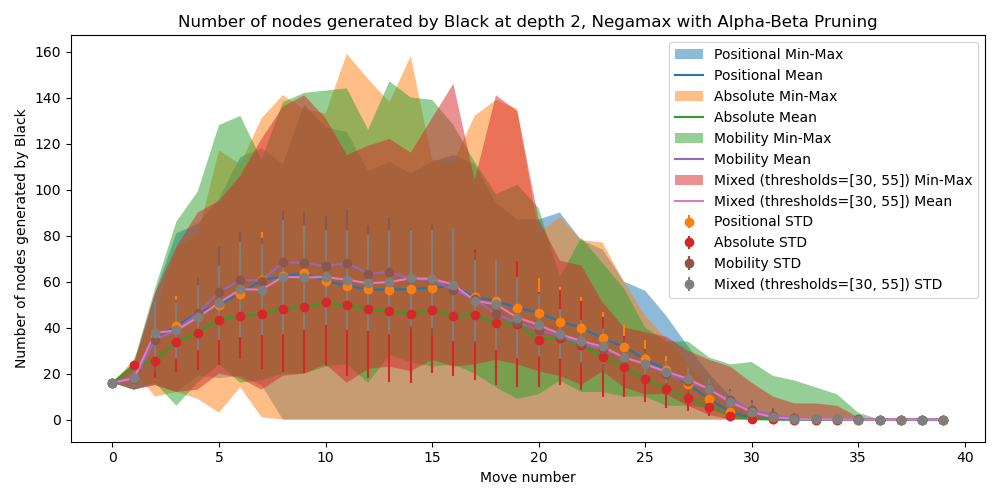
\includegraphics[width=1\textwidth]{ressources/Number of nodes generated by Black_depth_2_Negamax with Alpha-Beta Pruning.png}
    \caption{Nombre de noeuds explorés par coup pour la profondeur 2 avec Alpha-Beta.}
    \label{fig:node_explored_alpha_beta}
\end{figure}


\begin{figure}[H]
    \centering
    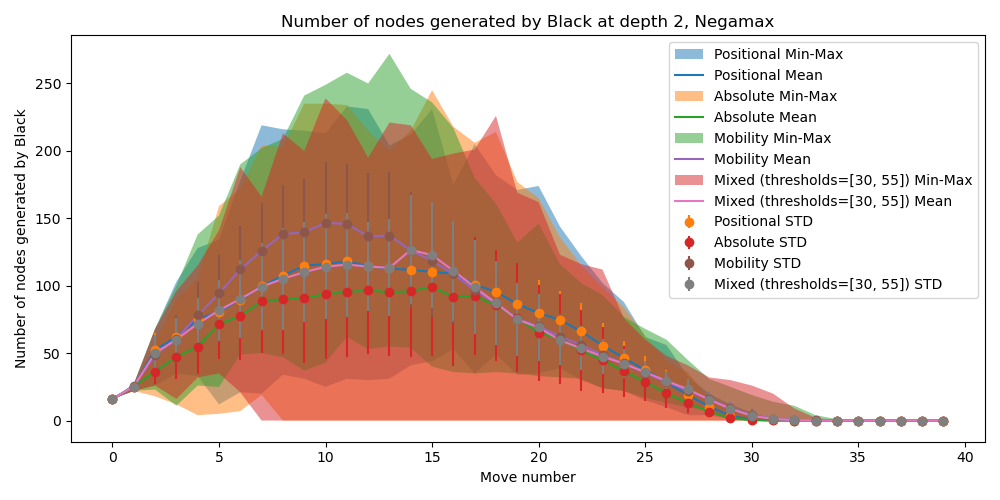
\includegraphics[width=1\textwidth]{ressources/Number of nodes generated by Black_depth_2_Negamax.png}
    \caption{Nombre de noeuds explorés par coup pour la profondeur 2 sans Alpha-Beta.}
    \label{fig:node_explored_negamax}
\end{figure}

\begin{figure}[H]
    \centering
    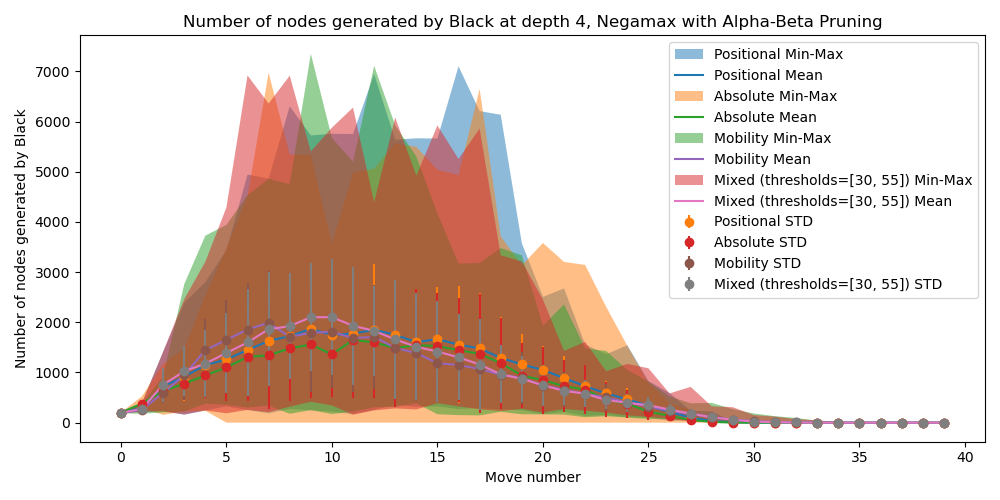
\includegraphics[width=1\textwidth]{ressources/Number of nodes generated by Black_depth_4_Negamax with Alpha-Beta Pruning.png}
    \caption{Nombre de noeuds explorés par coup pour la profondeur 4 avec Alpha-Beta.}
    \label{fig:node_explored_alpha_beta_4}
\end{figure}

\begin{figure}[H]
    \centering
    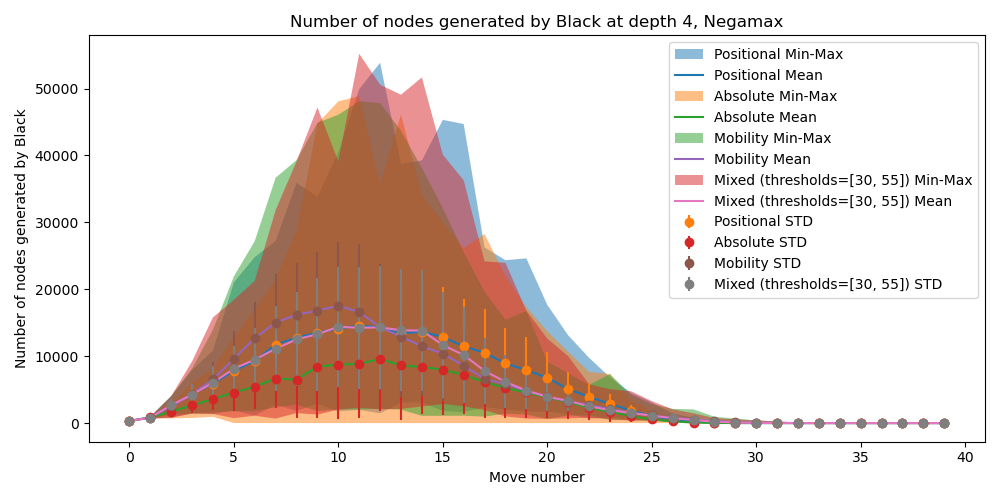
\includegraphics[width=1\textwidth]{ressources/Number of nodes generated by Black_depth_4_Negamax.png}
    \caption{Nombre de noeuds explorés par coup pour la profondeur 4 sans Alpha-Beta.}
    \label{fig:node_explored_negamax_4}
\end{figure}

\begin{figure}[H]
    \centering
    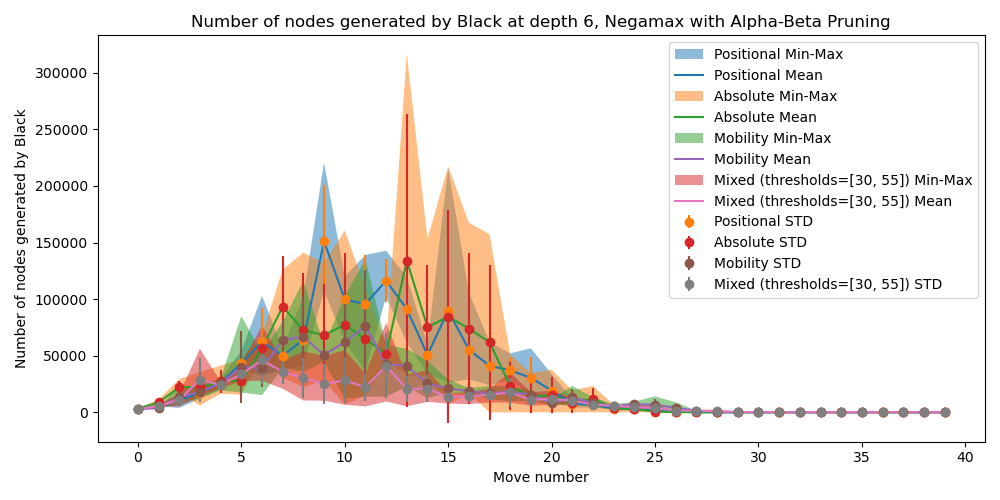
\includegraphics[width=1\textwidth]{ressources/Number of nodes generated by Black_depth_6_Negamax with Alpha-Beta Pruning.png}
    \caption{Nombre de noeuds explorés par coup pour la profondeur 6 avec Alpha-Beta.}
    \label{fig:node_explored_alpha_beta_6}
\end{figure}

\begin{figure}[H]
    \centering
    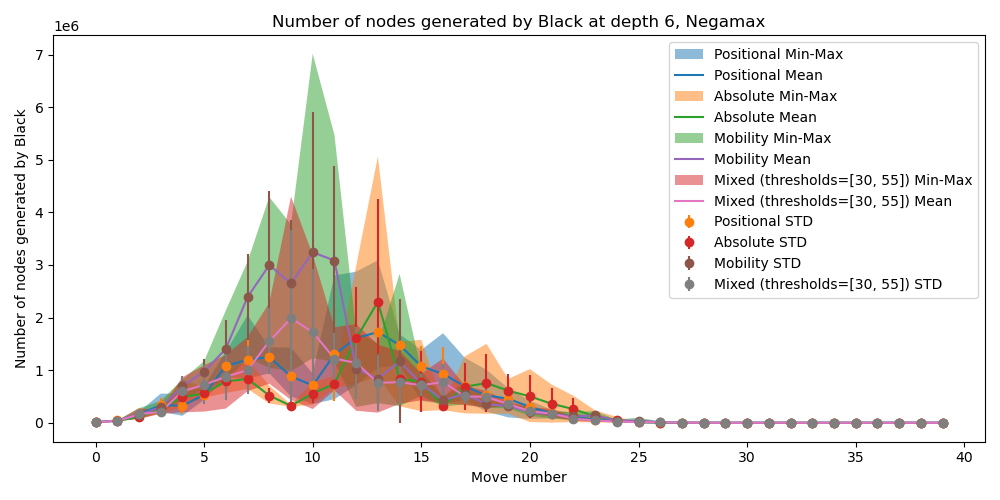
\includegraphics[width=1\textwidth]{ressources/Number of nodes generated by Black_depth_6_Negamax.png}
    \caption{Nombre de noeuds explorés par coup pour la profondeur 6 sans Alpha-Beta.}
    \label{fig:node_explored_negamax_6}
\end{figure}


\newpage

\pagenumbering{arabic}
\renewcommand{\thepage}{\arabic{page}}
\nocite{*}
\printbibliography

\newpage
\end{document}